%% LyX 2.3.2 created this file.  For more info, see http://www.lyx.org/.
%% Do not edit unless you really know what you are doing.
\documentclass[english]{article}
\usepackage[T1]{fontenc}
\usepackage[latin9]{inputenc}
\usepackage{graphicx}

\makeatletter

%%%%%%%%%%%%%%%%%%%%%%%%%%%%%% LyX specific LaTeX commands.
%% Because html converters don't know tabularnewline
\providecommand{\tabularnewline}{\\}

\makeatother

\usepackage{babel}
\begin{document}
\title{Practice 1 report}
\author{Guillermo Gir�n Garc�a}
\date{20 October 2019}
\maketitle
\begin{abstract}
Introducction to Turing Machines and RAM Model, with two examples
of problems that will be solved, analiced and compared.
\end{abstract}
%

\part*{Methodology}
\begin{itemize}
\item Utilization of Turing Machine Simulator.
\begin{itemize}
\item Developed at Princeton University.
\item Run over java.
\end{itemize}
\item Utilization of RAM Model simulator design by the teacher.
\item We will develop the solution for two problems, according to the simulator.
\item Then, the solutions we'll be analiced.
\item Another solutions we'll be design using the ram model tools provided
\item To conclude, they'll be compared through Cobham thesis.
\end{itemize}

\part*{Result and discussions}

To count steps in both ram problem implementations, I modified the
file given ``ram.h'' with a counter for every operation admited.

\section*{Palindrome problem}

\subsection*{Turing Machine}

I build a machine with only eight states that can solve the problem,
using an alphabet of two characters, \{0,1\}'s.

\includegraphics[scale=0.6]{\string"Maquinas de Turing/palindrome\string".png}

As we can see, for several input length values, between one and ten,
the graphics, fits perfectly at a polynomial grade two function.

The number of steps taken by every execution for $1\leq n\leq10$
are:

\begin{tabular}{|c|c|}
\hline 
input length & steps\tabularnewline
\hline 
\hline 
1 & 3\tabularnewline
\hline 
2 & 6\tabularnewline
\hline 
3 & 10\tabularnewline
\hline 
4 & 15\tabularnewline
\hline 
5 & 21\tabularnewline
\hline 
6 & 28\tabularnewline
\hline 
7 & 36\tabularnewline
\hline 
8 & 45\tabularnewline
\hline 
9 & 55\tabularnewline
\hline 
10 & 66\tabularnewline
\hline 
\end{tabular}

\subsection*{Ram Model}

For ram model implementation I created a program with seven labels,
that use eight registers to solve if any input string is a palindrome.

For input strings between $1\leq n\leq10$ it takes:

\begin{tabular}{|c|c|}
\hline 
input length & steps\tabularnewline
\hline 
\hline 
1 & 15\tabularnewline
\hline 
2 & 15\tabularnewline
\hline 
3 & 21\tabularnewline
\hline 
4 & 21\tabularnewline
\hline 
5 & 27\tabularnewline
\hline 
6 & 27\tabularnewline
\hline 
7 & 33\tabularnewline
\hline 
8 & 33\tabularnewline
\hline 
9 & 39\tabularnewline
\hline 
10 & 39\tabularnewline
\hline 
\end{tabular}

As we can see, results follow a clear pattern, increasing it number
of steps by six every time we increase the input length two units.
In this ocassion, the function does not fit perfectly any curve.

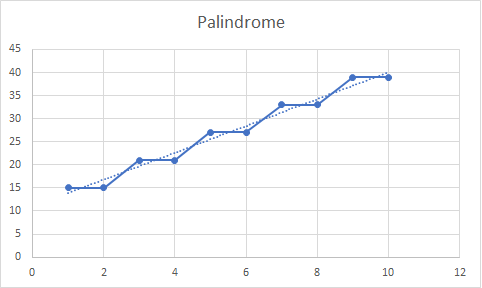
\includegraphics[scale=0.6]{Reports/palindromeram}

\section*{Binary comparator problem}

For this problem, input length is duplicated, due to the need of two
binary numbers to compare. This is taken in account during the analysis.

\subsection*{Turing Machine}

This time I build a machine with sixteen states that can solve the
problem, using a charachter alphabet, \{0,1,/\}, using '/' as a separator
of strings.

\includegraphics[scale=0.6]{\string"Maquinas de Turing/binary comparator\string".png}

In this ocassion the model fits too with a polynomial grade 2 function,
for inputs length values between one and ten.

The number of steps taken by every execution for $1\leq n\leq10$
are:

\begin{tabular}{|c|c|}
\hline 
input length & steps\tabularnewline
\hline 
\hline 
1 & 8\tabularnewline
\hline 
2 & 16\tabularnewline
\hline 
3 & 28\tabularnewline
\hline 
4 & 42\tabularnewline
\hline 
5 & 60\tabularnewline
\hline 
6 & 80\tabularnewline
\hline 
7 & 104\tabularnewline
\hline 
8 & 130\tabularnewline
\hline 
9 & 160\tabularnewline
\hline 
10 & 192\tabularnewline
\hline 
\end{tabular}

\subsection*{Ram Model}

To build a RAM model implementation of this problem I needed eight
labels with eight memory registers.

For input strings between $1\leq n\leq10$ it takes:

\begin{tabular}{|c|c|}
\hline 
input length & steps\tabularnewline
\hline 
\hline 
1 & 19\tabularnewline
\hline 
2 & 25\tabularnewline
\hline 
3 & 31\tabularnewline
\hline 
4 & 37\tabularnewline
\hline 
5 & 43\tabularnewline
\hline 
6 & 49\tabularnewline
\hline 
7 & 55\tabularnewline
\hline 
8 & 61\tabularnewline
\hline 
9 & 67\tabularnewline
\hline 
10 & 73\tabularnewline
\hline 
\end{tabular}

Its fair to say that the number of steps taken by the algorithm fits
a linear regresion.

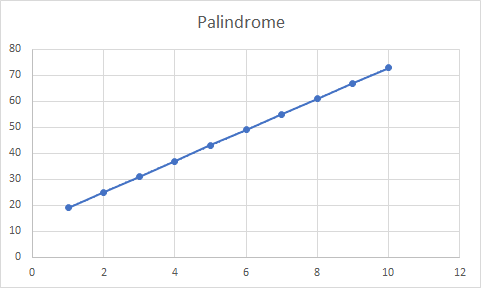
\includegraphics[scale=0.6]{Reports/comparatorram}

\section*{Conclusions}

In both cases RAM Model, appear to be more effective, having less
execution steps for high values of input length, however, for low
values, Turing machine seems to be more eficient.

Also, as can be checked, both problems can be solved in polynomial
time, so they both fulfill Cobham thesis requeriments.
\end{document}
